% Variante ohne Aufdeck-Effekte \documentclass[handout]{beamer}
% http://groups.google.de/group/comp.text.tex/browse_thread/thread/6ac8485c7a17252a
%\documentclass{beamer}
\documentclass[handout,draft]{beamer}
\usepackage[T1]{fontenc}
\usepackage[utf8]{inputenc}
\usepackage[ngerman]{babel}
\usepackage{listings}
\usepackage{color}

\mode<presentation>{\usetheme{Copenhagen}}

\title{Das Carrierpigeon-Projekt}
\author{Julius Adorf, Marek Kubica, Hong-Khoan Quach}

\date{13.11.2009\\ -  \\ETI-Projekt GP 8 \\ Sommersemester 2009}
\institute{Technische Universität München}

% Entfernen der Navigationsleiste
% Siehe auch http://wiki.ubuntuusers.de/ubuntuusers/LaTeX-Beamer
\beamertemplatenavigationsymbolsempty

% ftp://ftp.tex.ac.uk/tex-archive/macros/latex/.../listings/listings.pdf
\lstset{language=C}
\lstset{numbers=left}
\lstset{
    basicstyle=\small,
    keywordstyle=\color[rgb]{0.2,0.8,0.2}
    }

\begin{document}

\frame{\titlepage}

\frame{
    \frametitle{Gliederung}
    
    \begin{itemize}
        \item Idee
        \item Komponenten 
        \item Herausforderungen
        \item Ausblick 
    \end{itemize}
}

\frame{

    \frametitle{Idee}
    
    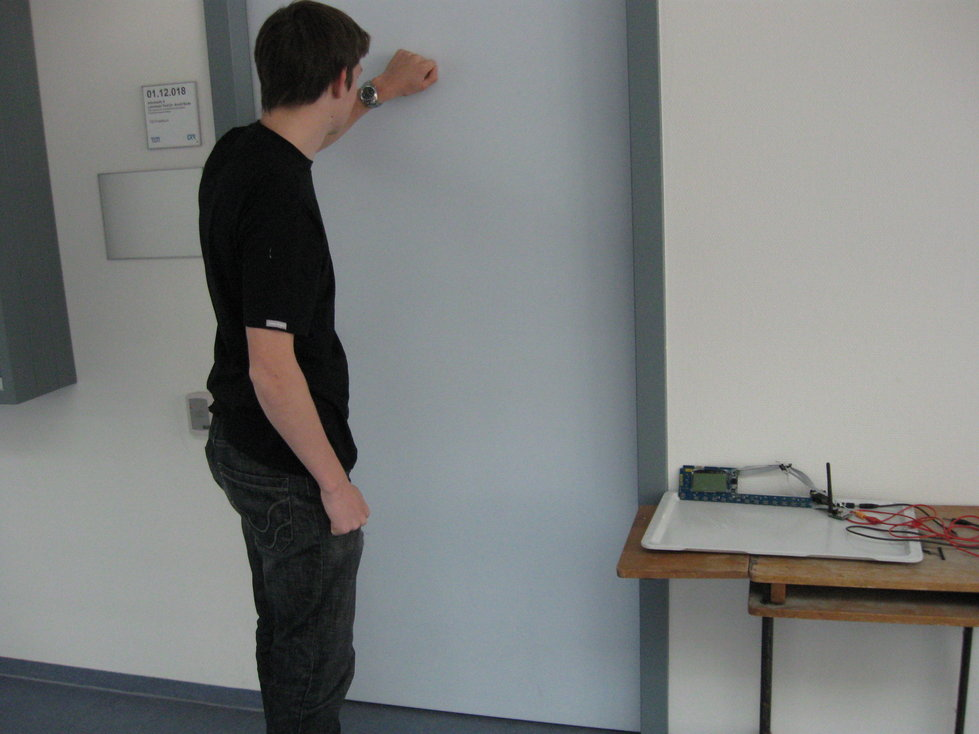
\includegraphics[scale=0.4]{media/story/1.JPG}
    \pause
    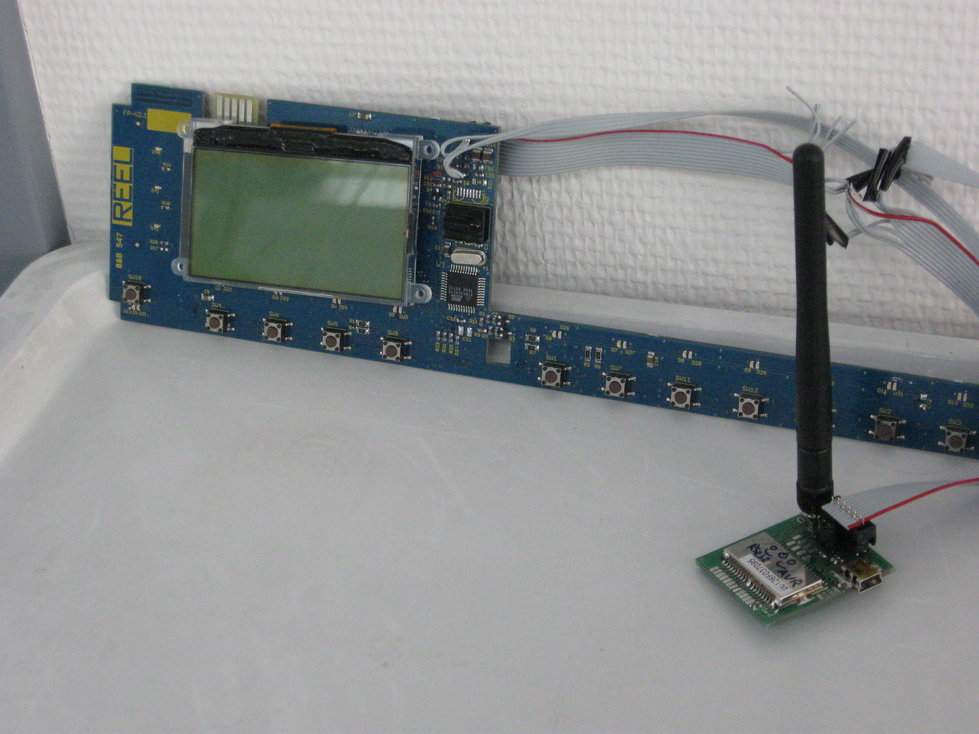
\includegraphics[scale=0.4]{media/story/2.JPG}\
    \pause
    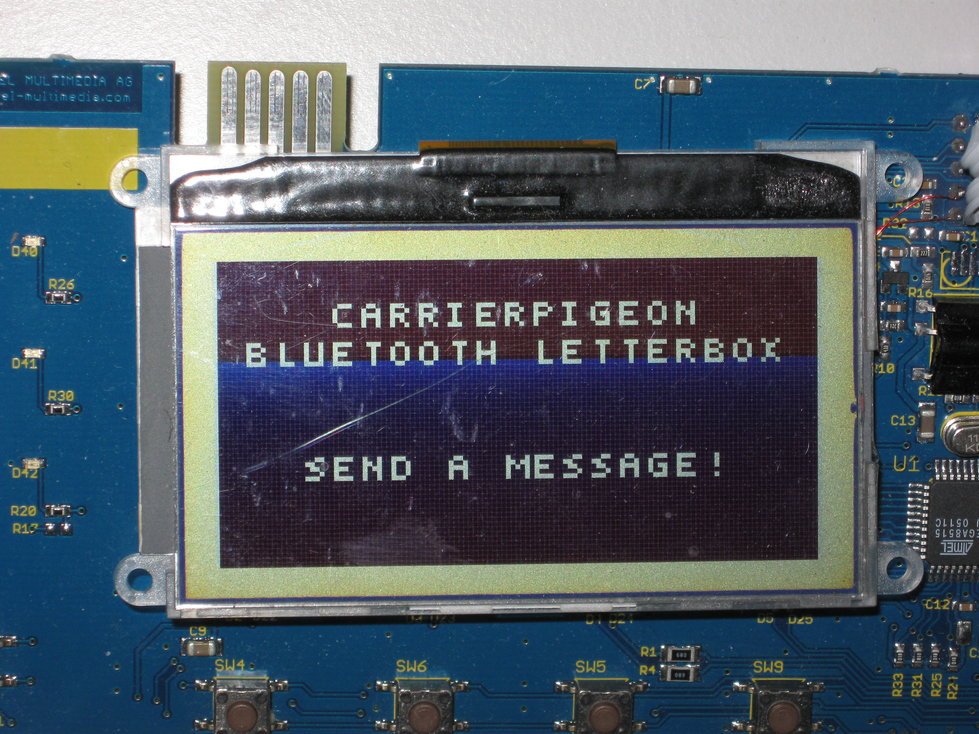
\includegraphics[scale=0.4]{media/story/3.JPG}
    
    
    %[pausesections] <- does not work....

}

\frame{
    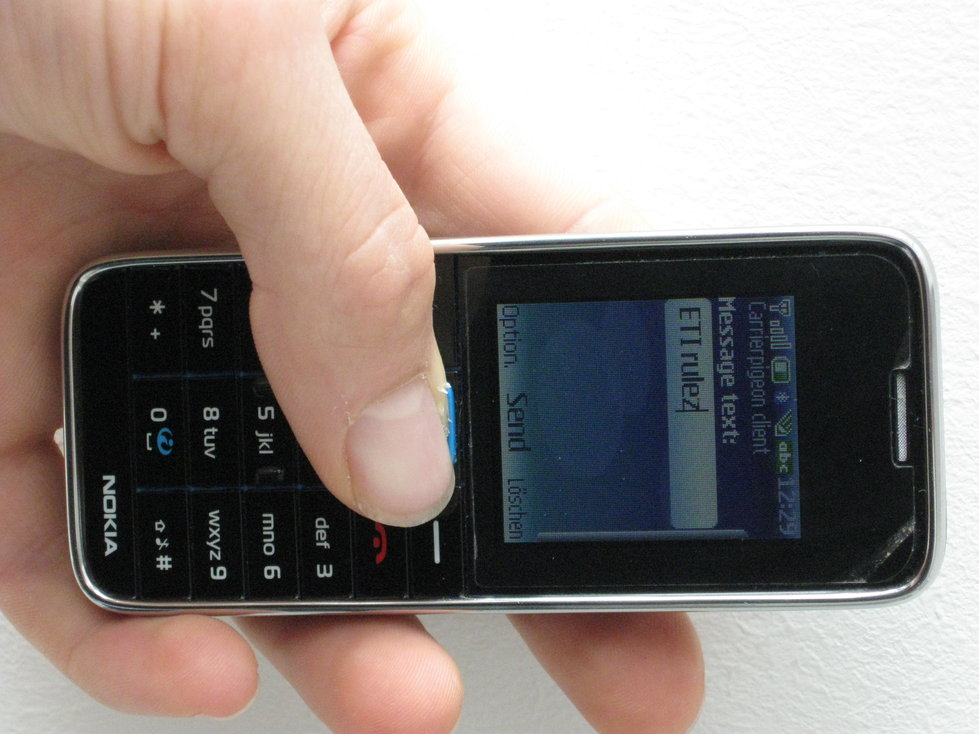
\includegraphics[angle=90, scale=0.5]{media/story/4.JPG}
    \pause
    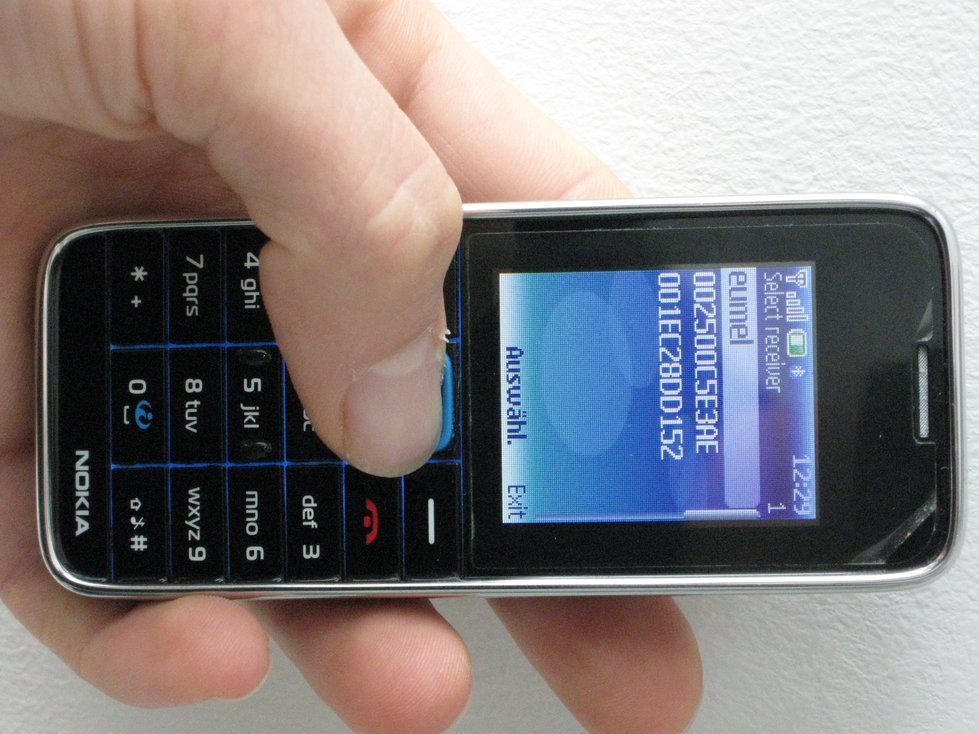
\includegraphics[angle=90, scale=0.5]{media/story/5.JPG}
    
    
}

\frame{
    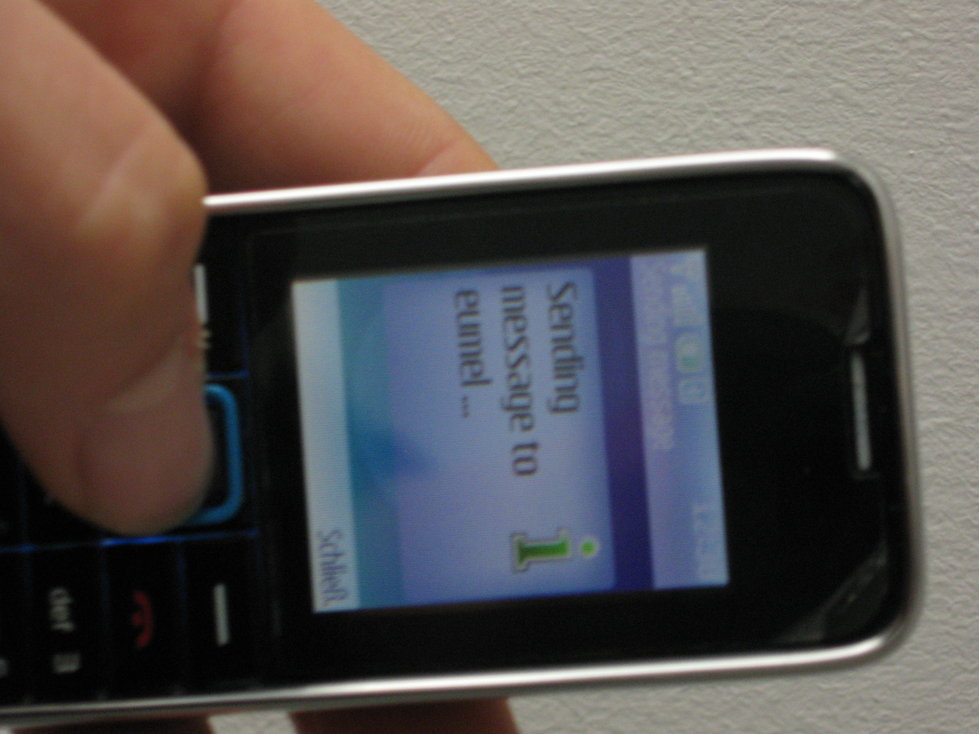
\includegraphics[angle=90, scale=0.5]{media/story/6.JPG}
    \pause
    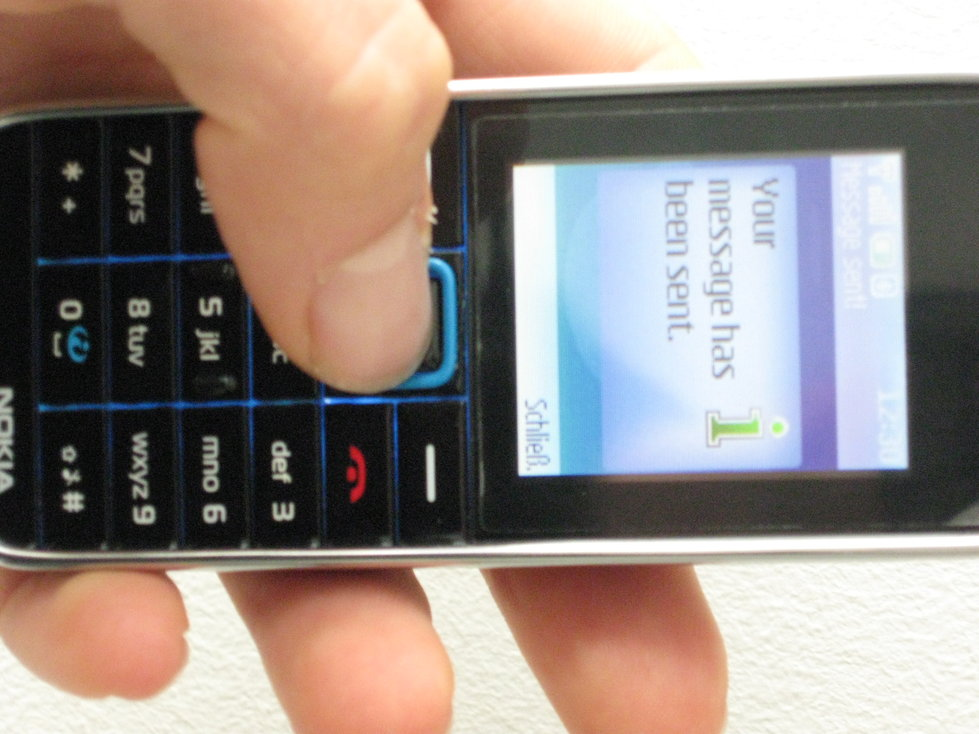
\includegraphics[angle=90, scale=0.5]{media/story/7.JPG}
}

\frame{
    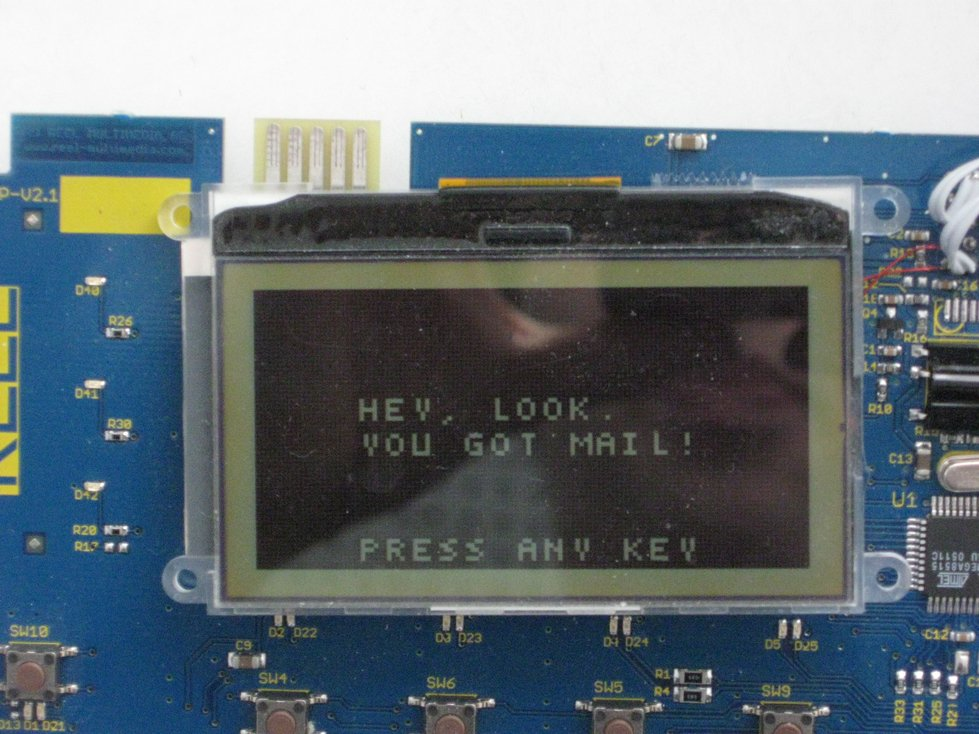
\includegraphics[scale=0.18]{media/story/8.JPG}\
    \pause
    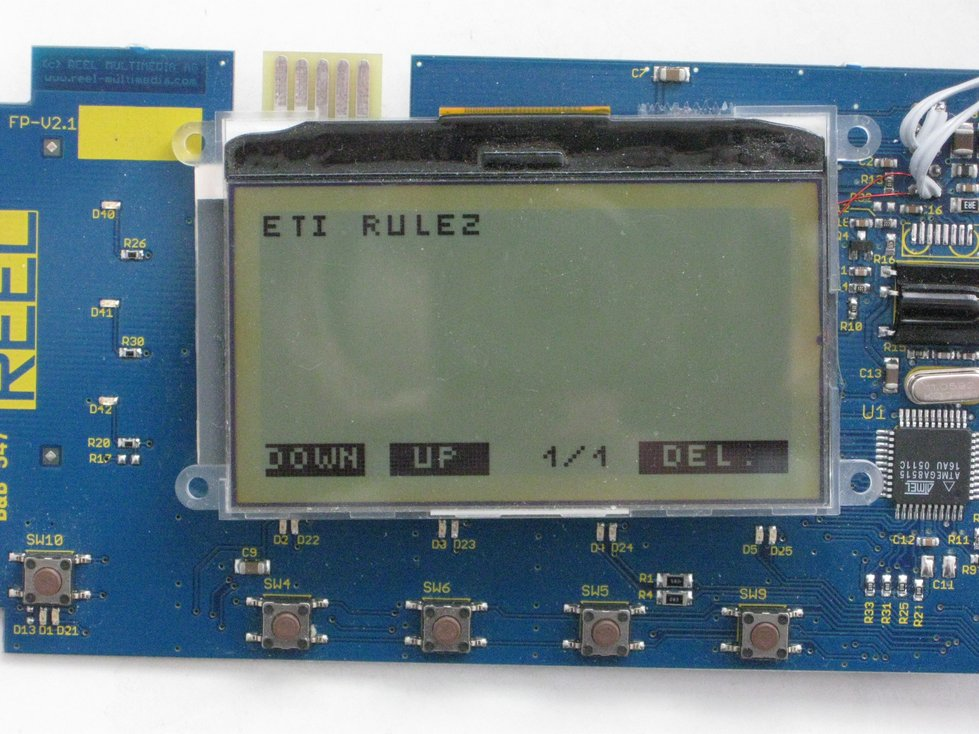
\includegraphics[scale=0.18]{media/story/9.JPG}\
}

\frame{
  \frametitle{Komponenten - Board}
  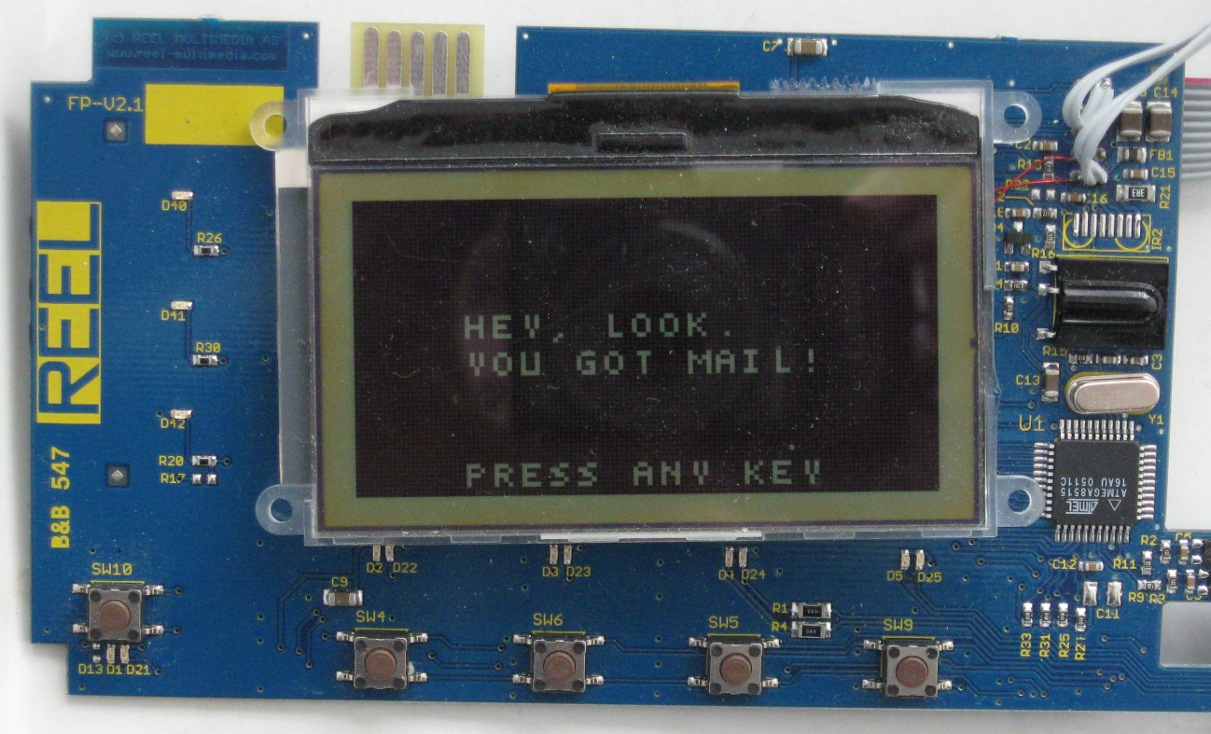
\includegraphics[scale=0.18]{media/board}
  \begin{block}{Mainboard}
    \begin{itemize}
      \item Mikrocontroller
      \item LEDs
      \item LCD
      \item Buttons
    \end{itemize}
  \end{block}
}

\frame{
  \frametitle{Komponenten - Bluetooth}
  \begin{columns}
    \column{0.4\textwidth}
      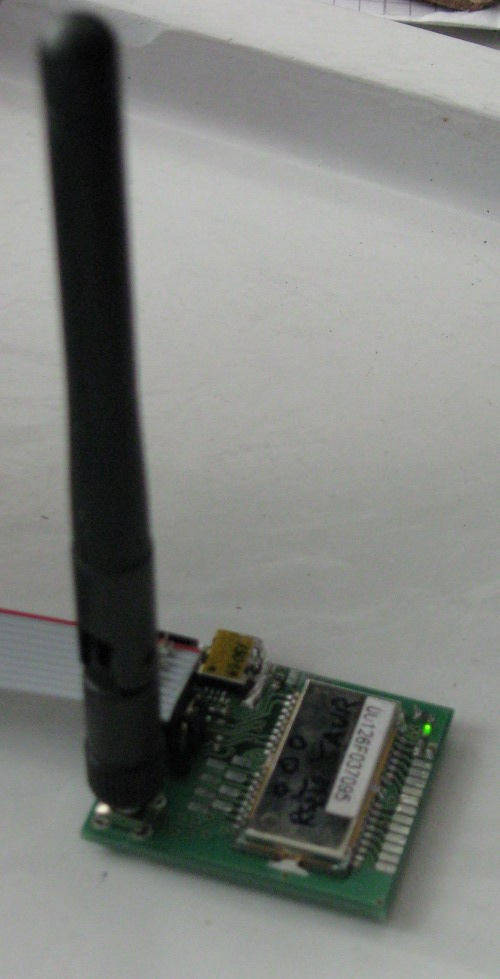
\includegraphics[scale=0.18]{media/bluetooth}
    \column{0.6\textwidth}
      \begin{block}{Antenne \& Controller}
        \begin{itemize}
          \item über UART ansprechbar
          \item kennt AT/Modem-Befehle
          \item kümmert sich selbst um die Verbindung
        \end{itemize}
      \end{block}
  \end{columns}
}

\frame{

    \frametitle{Herausforderung - Sicherheit und Stabilität}

    \begin{itemize}
        \item Bluetooth-Clients dürfen keinen Schaden anrichten 
        \item Programm darf nicht abstürzen 
        \item Neustart soll immer möglich sein
    \end{itemize}


    % 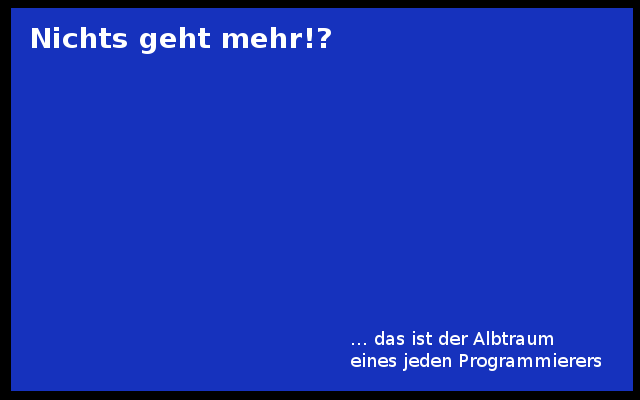
\includegraphics[scale=0.4]{media/bluescr}

}

\frame{
    \frametitle{Herausforderung - Sicherheit und Stabilität}

    \begin{itemize}
        \item der Server hat immer Recht 
        \item Timeouts sorgfältig programmiert
        \item Globale Variablen vermieden
        \item While-Schleifen vermieden
        \item While-Schleifen überprüft
    \end{itemize}

}

\frame{

    \frametitle{Herausforderung - Speicherverwaltung}

    \includegraphics[scale=0.4]{media/eeprom}

}

\frame{
    
    \frametitle{Herausforderung - Speicherverwaltung}

   \begin{itemize}
        \item Nachrichtenzähler überprüfen
        \item Blockzeiger überprüfen
        \item Blockzeiger auf Duplikate überprüfen
    \end{itemize}

    Damit der Techniker nicht zum Hausbesuch kommen muss.

}

\frame{
    \frametitle{Herausforderung - Speichermangel}

    \begin{block}{Die Hardware}

      \begin{tabular}{|l|l|}
        \hline
        Flash & 8 KB \\
        EEPROM & 512 Byte \\
        SRAM & 512 Byte \\
        \hline
      \end{tabular}

      \begin{itemize}
        \item ATmega8515, 8-Bit AVR-MCU
	\item 512 Byte = 512 Zeichen!
	\item Harvard-Architektur
      \end{itemize}
    \end{block}
}

\frame{
   \frametitle{Herausforderung - Komisches Verhalten}

   \begin{block}{Bugs}
     \begin{itemize}
       \item Stack und Heap kollidieren
       \item Unerklärliches Verhalten
       \item Heisenbugs
     \end{itemize}
   \end{block}

   \begin{block}{Diagnose}
     \begin{itemize}
       \item \texttt{avr-size} gibt Gesamtspeicher aus
       \item \texttt{avr-nm} gibt Speicherverbrauch granular aus
       \item Distanz von Stack (\texttt{SP}) und Heap (\texttt{\&\_\_heap\_start}) ermittelbar
     \end{itemize}
   \end{block}
}

\frame{
    \frametitle{Herausforderung - Speicher sparen}

    \begin{block}{Dynamische Speicherverwaltung}
      \begin{itemize}
        \item Nur Strings allokieren die wir brauchen
	\item Funktioniert nicht, Heisenbugparade
      \end{itemize}
    \end{block}

    \begin{block}{Buffer sharing}
      \begin{itemize}
        \item Vorher: jeder Programmteil eigene Buffer
	\item Nachher: alles über globalen Buffer
      \end{itemize}
    \end{block}

    \begin{block}{Harvard ausnutzen}
      \begin{itemize}
        \item Zeichenmapping verbraucht viel RAM (235 Bytes)
        \item \texttt{PROGMEM}-Erweiterung des AVR-GCC
      \end{itemize}
    \end{block}
}

\frame{
    \frametitle{Herausforderung - LC-Display und Textausgabe}
    
    \begin{itemize}
        \item Punkt ausgeben
        \item Buchstaben (8x5 Matrix)
        \begin{figure}
            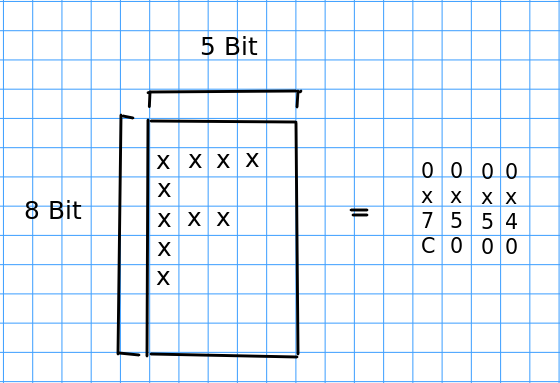
\includegraphics[scale=0.35]{media/char.png}
        \end{figure}
        \item Text verkehrt rum
     \end{itemize}
     
     %\begin{flushright}
      %  \begin{figure}
       % 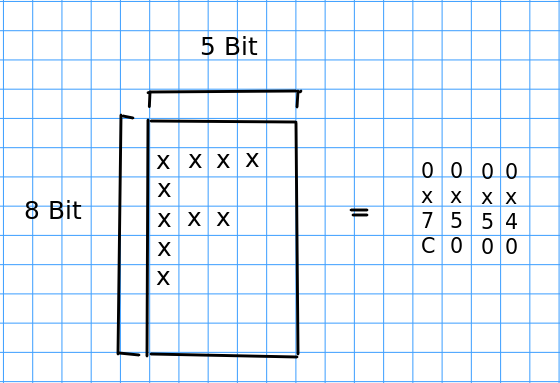
\includegraphics[scale=0.2]{media/char.png}
        %\end{figure}
     %\end{flushright}
     
     $\Rightarrow$ Handbücher ganz genau lesen
}

\frame{

    \frametitle{Ausblick - Ausbaumöglichkeiten}

\begin{figure}
    \includegraphics[scale=0.2]{media/idea}
\end{figure}

   \begin{itemize}
        \item Protokollerweiterung 
        \item Mehr Speicher einbauen 
        \item Korrekte Zeilenumbrüche
        \item Automatische Tests mit GNU Debugger und AVR-Simulator 
    \end{itemize}

}

\frame{

    \frametitle{Ausblick - Alternativen}

    \begin{center}
        Alternative Entwicklung:

        \begin{figure}
            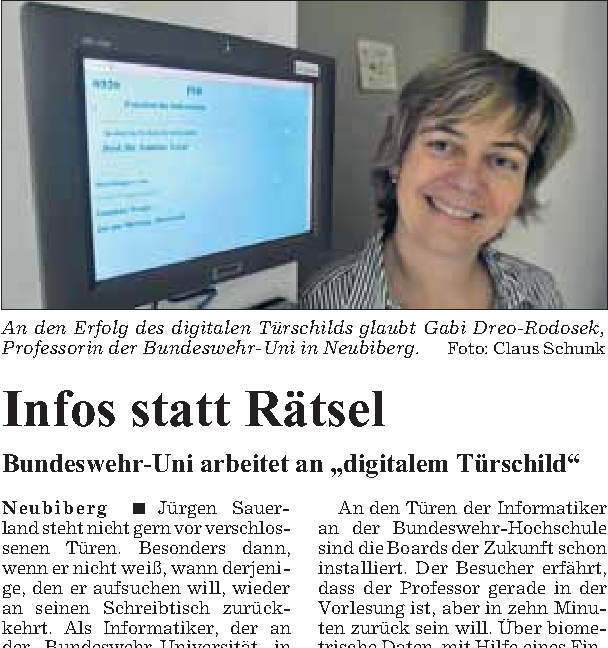
\includegraphics[scale=0.4]{media/tuerschild-sz-small}
        \end{figure}

        (Süddeutsche Zeitung, 12.11.2009)
    \end{center}

}

\frame{

    \frametitle{Ausblick - Fazit}

    \begin{figure}
        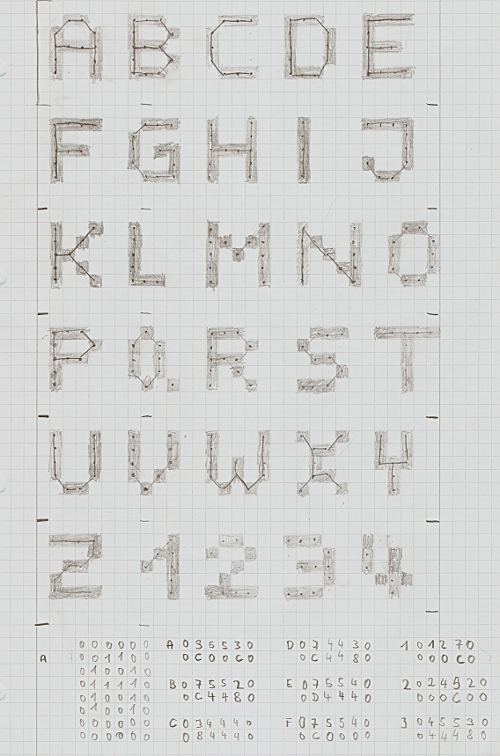
\includegraphics[scale=0.6]{media/font}
    \end{figure}

   \begin{itemize}
        \item Anforderungen erfüllt!
        \item Einsatz verschiedener Techniken ...
        \item ... was am Ende auch funktioniert hat!
    \end{itemize}

}

\frame{

    \frametitle{Ausblick -- Ausprobieren}

    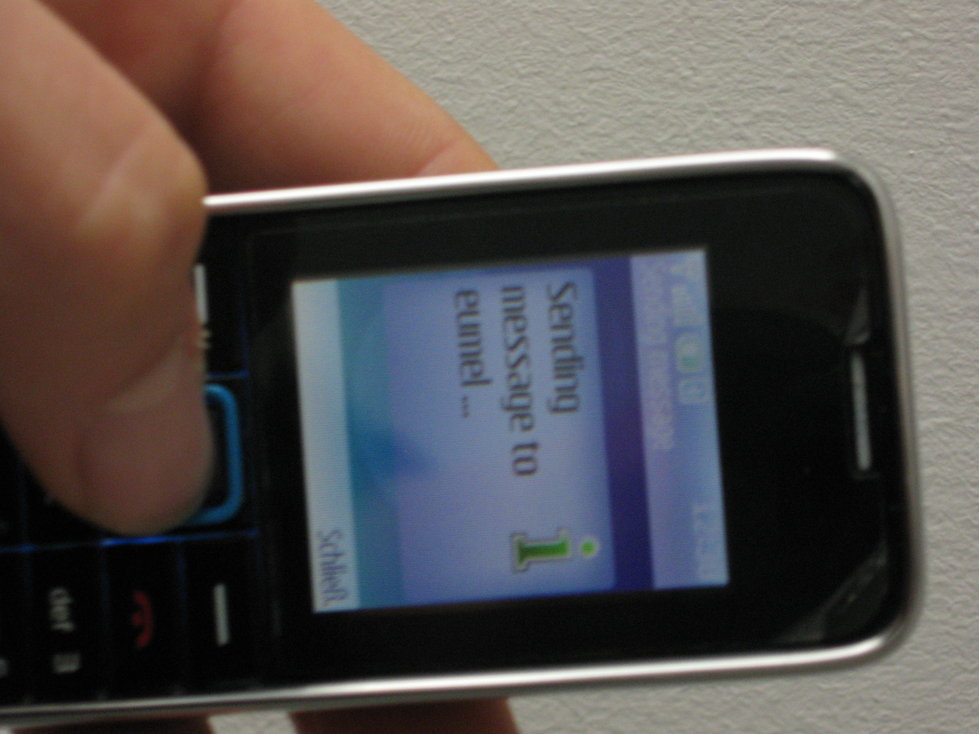
\includegraphics[angle=90, scale=0.24]{media/story/6.JPG}

    Wer es ausprobieren mag:

   \begin{itemize}
        \item http://bitbucket.org/jeadorf/carrierpigeon/downloads
        \item Mobile-Client (JAR und evtl. JAD) herunterladen und auf das Handy spielen
    \end{itemize}

}

%
% --------------------------

\frame{

    \frametitle{Toolchain}


    \begin{tabular}{|r||l|}
        \hline
        Hardware & ATmega 8515, BTM-222, ST7565 LCD, AVRISP2 \\
        \hline
        Languages & C, Java, Python\\
        \hline
        Framework & Java Micro Edition, Peter Fleury's UART library\\
        \hline
        Compilation & {\tt avr-gcc, avr-objcopy, avr-strip, avrdude,} \\
                    & {\tt avr-nm, avr-size, splint, python, ant} \\
        \hline
        Helpers & {\tt hcitool, rfcomm, gtkterm, jpnevulator} \\
        \hline
    \end{tabular}

    
}

\end{document}

